Calcular la energía cinética que lleva una bala de 0.006 kg si su velocidad posee una magnitud de 510 m/s.

\begin{minipage}{0.3\textwidth}
    \begin{figure}[H]
        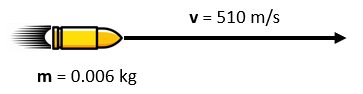
\includegraphics[width=\linewidth]{../images/energia_cinetica_problema_1.png}
    \end{figure}
\end{minipage}\hfill
\begin{minipage}{0.65\textwidth}
    \begin{solutionbox}{6cm}
        \begin{multicols}{2}
            Datos:

            Ec = ?

            m = 0.006 kg

            v = 510 m/s

            La energía cinética es:
            \[E_c=\frac{1}{2}mv^2\]

            \vspace{2cm}

            Sustituyendo nuestros datos en la fórmula:
            \[
                \begin{array}{rl}
                    E_c & = \dfrac{1}{2} (0.006 \text{ kg})(510 \text{ m/s})^2  \\[1em]
                        & = 0.5 (0.006 \text{ kg})(260,100 \text{ m$^2$/s$^2$}) \\[1em]
                        & =780.3 \text{ J }
                \end{array}
            \]
        \end{multicols}
        \begin{center}Obtenemos una energía cinética de 780.3 J.\end{center}
    \end{solutionbox}
\end{minipage}